% chapters/glitch.tex
%
% Copyright 2023 Alexander Lyttle.
%
% This work may be distributed and/or modified under the conditions of the
% LaTeX Project Public License (LPPL) version 1.3 or later.
%
% The latest version of this license is in
% https://www.latex-project.org/lppl.txt and version 1.3 or later is part of
% all distributions of LaTeX version 2005/12/01 or later.
%
%
\chapter[Acoustic glitches]{Acoustic glitches as a signature of helium abundance}\label{chap:glitch}

A glitch arises from a sharp structural variation in the star.

Explain that glitches can be a signature of helium abundance. If we can model the glitch consistently between models and observed stars, we can add parameters to the HBM which contain information about helium.

In this chapter, we explore the theoretical background of acoustic glitches

\section[1D example]{A one-dimensional example of a glitch}

A rapid variation in the structure of a medium induces an oscillation in the eigenfrequencies, \(\delta\omega\). To demonstrate this, we will explore a simple one-dimensional example. Consider a medium bound from \(x=0\) to \(x=L\) in which pressure waves can propagate at constant speed \(c\). The longitudinal displacement of the wave \(\xi\) must obey the wave equation,
%
\begin{equation}
    \frac{\partial^2\xi(x, t)}{\partial t^2} = c^2 \frac{\partial^2\xi(x, t)}{\partial x^2},
\end{equation}
%
at a given position \(x\) and time \(t\). A general solution to the wave may be written as a sum of right- and left-travelling waves. In terms of the angular frequency \(\omega\), wave number \(k\), and complex coefficients \((A, B)\),
%
\begin{equation}
    \xi(x, t) = A e^{i (\omega t - k x)} + B e^{i (\omega t + k x)},
\end{equation}
%
where \(\omega\) and \(k\) satisfy \(\omega = c k\). Solving for the boundary condition \(\xi(0, t) = 0\) we find \(B = - A\). Substituting \(A = (r/2) e^{i\phi}\) we can write the real solution for \(\xi\) as,
%
\begin{equation}
    \real\left[\xi(x, t)\right] = r \sin k x \sin(\omega t + \phi),
\end{equation}
%
where \(r\) and \(\phi\) are the amplitude and temporal phase respectively. Solutions for \(\omega\) which satisfy \(\xi(L, t)=0\) may then be found,
%
\begin{equation}
    \omega_n = c \frac{n \pi}{L}, \label{eq:omega-n}
\end{equation}
%
where \(n\) is a non-zero integer (the \(n=0\) solution would give \(\xi=0\) everywhere).

Now, let us suppose there is a small structural perturbation (or glitch) in the medium at position \(x_0\) with half-width \(\delta x\). Figure \ref{fig:1d-diagram} shows this system divided into 3 regions, with region 2 containing the glitch. In region 2, the speed of sound is \(c + \delta c\) and the corresponding wave number is \(k + \delta k\). We want to find the frequencies which correspond to standing waves in this system and compare them to that of the homogeneous medium above. We will show that the resulting eigenfrequencies oscillate with an amplitude and period that relates to the properties of the glitch.

Firstly, we propose solutions to the wave for each region by considering reflection and transmission at each boundary. Initially ignoring the wave superposed by a reflection at \(x=L\),
%
\begin{align}
    \xi_1(x, t) &= e^{i(\omega t - k x)} + A e^{i(\omega t + k x)}, \label{eq:xi1-r} \\
    \xi_2(x, t) &= Be^{i(\omega t - (k + \delta k) x)} + C e^{i(\omega t + (k + \delta k) x)}, \label{eq:xi2-r} \\
    \xi_3(x, t) &= D e^{i(\omega t - k x)}, \label{eq:xi3-r}
\end{align}
%
where complex coefficients \(A\) and \(C\) represent reflections, and \(B\) and \(D\) represent transmissions, at \(x_0 \pm \delta x\) respectively. Later, we will substitute the left-travelling wave (\(- \xi\{-k, -\delta k\}\)) after determining the values of the coefficients.

\begin{figure}
    \centering
    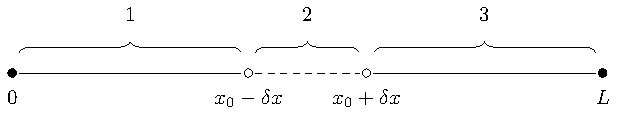
\includegraphics{figures/glitch-1d-example-diagram.pdf}
    \caption[A diagram showing a one-dimensional medium with a small structural perturbation.]{A diagram showing a one-dimensional medium split into three regions. 1: Fixed at \(x=0\) with a constant speed of sound \(c\); 2: A small structural perturbation centred at \(x=x_0\) with width \(2\delta x\) and constant speed of sound \(c + \delta c\); 3: Fixed at \(x=L\) with a constant speed of sound \(c\).}
    \label{fig:1d-diagram}
\end{figure}

The boundary conditions for this system are,
%
\begin{align*}
    \xi_1(x_0 - \delta x, t) &= \xi_2(x_0 - \delta x, t), \\
    \xi_2(x_0 + \delta x, t) &= \xi_3(x_0 + \delta x, t), \\
    \frac{\partial \xi_1}{\partial x}(x_0 - \delta x, t) &= \frac{\partial \xi_2}{\partial x}(x_0 - \delta x, t), \\
    \frac{\partial \xi_2}{\partial x}(x_0 + \delta x, t) &= \frac{\partial \xi_3}{\partial x}(x_0 + \delta x, t).
\end{align*}
%
Solving these simultaneously gives the following equations for the complex coefficients,
%
\begin{align}
    A &= \delta k (2k + \delta k) (1 - e^{4i \delta x (k + \delta k)}) e^{- 2i k (x_0 - \delta x)} \alpha^{-1}, \\
    B &= 2 k (2k + \delta_k) e^{4i \delta x (k + \delta k)} e^{i \delta k (x_0 - \delta x)} \alpha^{-1}, \\
    C &= 2 k \delta k e^{- i (x_0 - \delta x) (2k + \delta k)} \alpha^{-1}, \\
    D &= 4 k (k + \delta k) e^{2 i \delta x (2k + \delta k)} \alpha^{-1},
\end{align}
%
where,
\begin{equation}
    \alpha = (2k + \delta k)^2 e^{4 i \delta x (k + \delta k)} - \delta k^2.
\end{equation}
%

Now we have solutions for the coefficients, we can superpose the right-travelling wave, \(\xi\{k, \delta k\} \rightarrow - \xi\{-k, -\delta k\}\) to get the full solution for the wave function. Substituting \(k \rightarrow -k\) and \(\delta k \rightarrow -\delta k\) into the coefficients yields their complex conjugates, \((\overline{A},\overline{B},\overline{C},\overline{D})\). This allows us to rewrite the wave functions into a more flexible form. For example, substituting Euler's formula, \(A = (r_A/2) e^{i\phi_A}\) and \(\overline{A} = (r_A/2) e^{-i\phi_A}\), Equation \ref{eq:xi1-r} now becomes,
%
\begin{equation}
    \xi_1(x, t) = e^{i \omega t} \left[ \frac{r_A}{2} \left( e^{i(kx + \phi_A)} - e^{-i(kx + \phi_A)} \right) - \left( e^{ikx} - e^{-ikx} \right) \right] \label{eq:xi1}
\end{equation}
%
where its real component is,
\begin{equation}
    \real\left[\xi_1(x, t)\right] = \sin \omega t \left[2 \sin kx - r_A \sin(kx + \phi_A)\right].
\end{equation}
%
However, this does not satisfy the boundary condition that \(\xi_1(0, t) = 0\). To do so, we must introduce a small displacement phase \(\epsilon\) and let \(x \rightarrow x + \epsilon\). We will determine \(\epsilon\) shortly. In the meantime, superposing the right-travelling wave and substituting Euler's formula into Equations \ref{eq:xi2-r} and \ref{eq:xi3-r}, we get the real components of the wave functions,
%
% \begin{align}
%     \xi_3(x, t) = \frac{r_A}{2} e^{i \omega t} \left[ e^{i(k(x + \epsilon) + \phi_A)} - e^{-i(k(x + \epsilon) + \phi_A)} \right],
% \end{align}
%
% with a real solution in trigonometric form,
%
\begin{align}
    \real[\xi_1(x, t)] &= \sin \omega t \left\{2 \sin[k (x + \epsilon)] - r_A \sin[k(x + \epsilon) - \phi_A]\right\} \label{eq:xi1-real} \\
    \real[\xi_2(x, t)] &= \sin \omega t \left\{ r_B \sin[(k + \delta k)(x + \epsilon) - \phi_B] - r_C \sin[(k + \delta k)(x + \epsilon) - \phi_C]\right\} \\
    \real[\xi_3(x, t)] &= \sin \omega t \left\{r_D \sin[k(x + \epsilon) - \phi_D]\right\} \label{eq:xi3-real}
\end{align}
%
Imposing the boundary condition \(\xi_1(0, t) = 0\), we solve Equation \ref{eq:xi1-real} for \(\epsilon\) at \(x=0\),
%
\begin{align}
    \epsilon &= \frac{1}{k} \tan^{-1}\left( \frac{(r_A / 2) \sin(\phi_A)}{1 - (r_A/2) \cos(\phi_A)} \right), \notag\\
    &= \frac{1}{k} \tan^{-1}\left( \frac{\imag[A]}{1 - \real[A]} \right). \label{eq:1d-phase}
\end{align}
%

Finally, we can impose the boundary condition \(\xi_3(L, t) = 0\) to solve for \(\omega\). Setting Equation \ref{eq:xi3-real} to zero, we can rewrite it in terms of the real and imaginary components of \(D\),
%
\begin{align}
    \sin \omega t \left\{r_D \sin[k(L + \epsilon) - \phi_D]\right\} &= 0, \quad (\div \sin \omega t) \notag \\
    r_D \cos \phi_D \sin[k(L + \epsilon)] - r_D \sin \phi_D \cos[k(L + \epsilon)] &= 0, \notag \\
    \real[D] \sin[k(L + \epsilon)] - \imag[D] \cos[k(L + \epsilon)] &=0. \label{eq:1d-glitch-sol}
\end{align}
%
Unfortunately, solving Equation \ref{eq:1d-glitch-sol} for \(\omega\) is not possible analytically. However, we can find individual modes (\(\omega_n\)) numerically.

We find \(\omega_n\) by solving Equation \ref{eq:1d-glitch-sol} using Newton's method for \(n = 1,\dots,50\), with \(c=1\), \(L=1\), and several values of \(x_0\), \(\delta x\), and \(\delta c\). Initial guesses are obtained from the homogeneous medium solutions in Equation \ref{eq:omega-n}. The difference between the solutions for \(\omega_n\) and those from the homogeneous medium are shown in Figure \ref{fig:1d-results}. We can see that the change in frequency (\(\delta \omega\)) induced by the glitch oscillates. There appears to be a linear component and a short period oscillation modulated by a longer period. As the location of the glitch (\(x_0\)) increases towards the edge of the system, the short-period oscillation of \(\delta\omega\) increases. Similarly, as the the half-width of the glitch (\(\delta x\)) increases, the longer modulation period increases. Furthermore, an increasing change in sound speed (\(\delta c\)) increases the amplitude of \(\delta\omega\). Finally, increasing both \(\delta x\) and \(\delta c\) increases the slope of \(\delta\omega\).

\begin{figure}
    \centering
    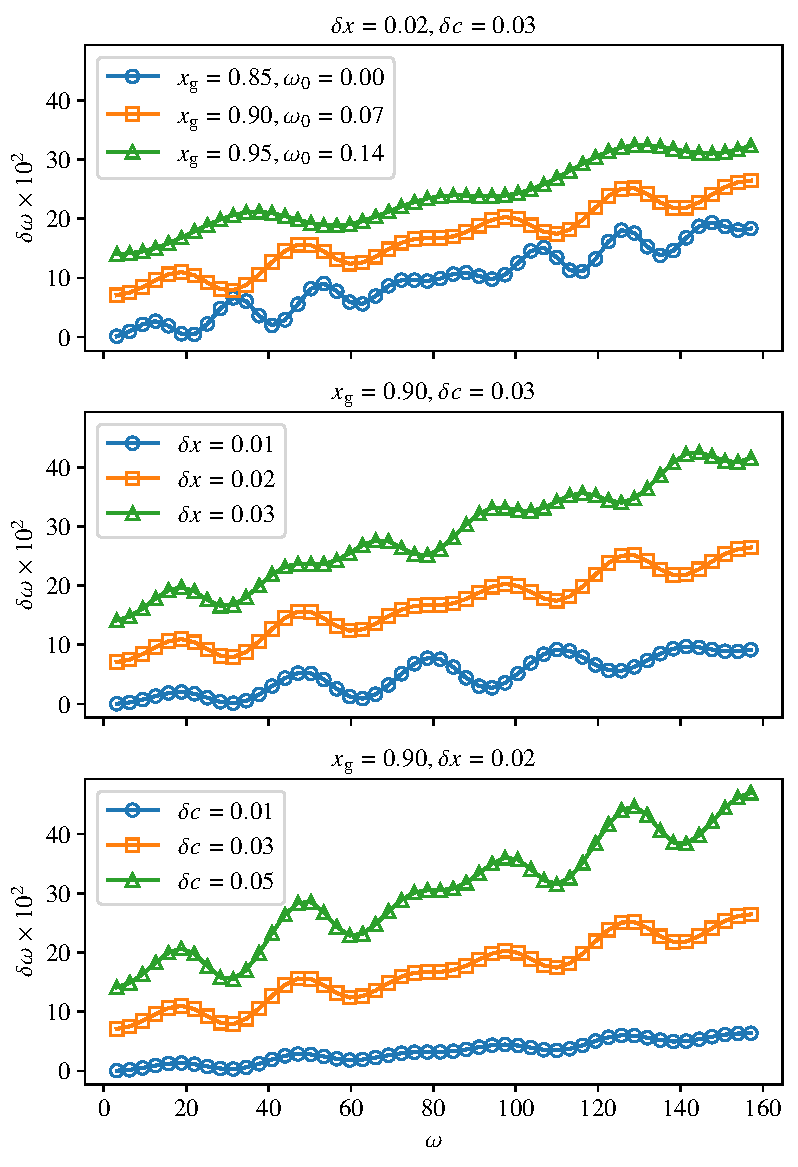
\includegraphics{figures/glitch-1d-example-results.pdf}
    \caption{The change in mode frequency induced by a change in sound speed of \(\delta c\) from \(x=x_0\) to \(x=x_0 + \delta x\) in a one-dimensional medium, bound such that \(x \in [0, 1]\) (see Figure \ref{fig:1d-diagram}). Outside of the perturbation the speed of sound, \(c=1\).
    The frequencies in the top panel are offset by \(\omega_0\).
    }
    \label{fig:1d-results}
\end{figure}

%This may be interpreted as the nodes of each standing wave passing in and out of region 2 with increasing \(n\). Where there is a node, the wave is least sensitive to a change in structure, and 

The small phase offset \(\epsilon\) in Equation \ref{eq:1d-phase} is required for the wave function to satisfy the boundary conditions at \(x = 0\). However, adding \(\epsilon\) shifts the effective location of \(x_0\). We plot \(\epsilon\) against \(\omega\) in Figure \ref{fig:1d-phase} and show that its magnitude is \(\sim 10^{-4}\), much smaller than the location and size of region 2. The oscillation caused by the glitch also shows up in Figure \ref{fig:1d-phase}, with its properties affected in a similar way to Figure \ref{fig:1d-results}.

\begin{figure}
    \centering
    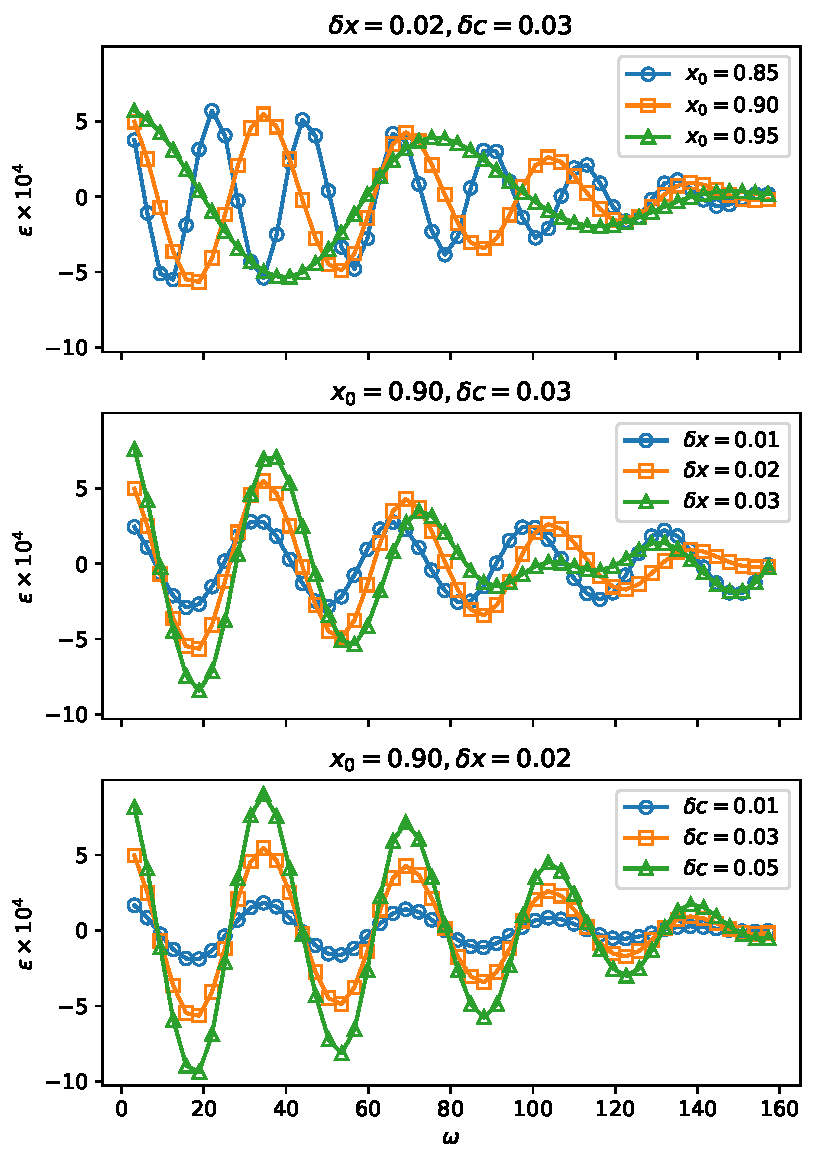
\includegraphics{figures/glitch-1d-example-phase.pdf}
    \caption{The same as Figure \ref{fig:1d-results} but showing the phase offset \(\epsilon\) required to satisfy the boundary conditions.}
    \label{fig:1d-phase}
\end{figure}

Finding an approximate solution for \(\delta\omega\) is beyond the scope of this simple example. However, we can show that by modelling \(\delta\omega\), we can recover information about the structural glitch. Let us build a model \(\delta\omega = f(\omega)\). Looking at Figure \ref{fig:1d-results}, we propose a form for \(f\),
%
\begin{equation}
    f(\omega) = a_1 \omega - a_2 \sin (\tau_1 \omega) \cos (\tau_2 \omega), \label{eq:1d-domega-func}
\end{equation}
%
where \(a_1\) and \(a_2\) are coefficients which are both functions of \(\delta x\) and \(\delta c\). Parameters \(\tau_1\) and \(\tau_2\) are the `frequencies' (units of time\footnote{A frequency in \(\omega\) would have units of time, but shouldn't be confused with a periodicity in \(\omega\).}) of oscillations in \(\delta\omega\), which are functions of \(\delta x\) and \(x_0\) respectively.

We fit Equation \ref{eq:1d-domega-func} to \(\delta\omega_n\) obtained from a glitch located at \(x_0 = 0.9\), with half-width \(\delta x = 0.02\), and change in sound speed \(\delta c = 0.03\). The best fitting line is shown in Figure \ref{fig:1d-fit}. Repeating this for different glitch parameters, it can be shown empirically how the `frequencies' \(\tau_1\) and \(\tau_2\) relate to the half-width and location of the glitch respectively. It emerges that \(\tau_1 \approx 2\delta\tau\), where \(\delta\tau\) is half the acoustic width of the glitch (i.e. the time at which sound takes to transverse the region). The second `frequency' \(\tau_2 \approx 2\tau_0\), where \(\tau_0\) is the acoustic depth from the nearest edge to the centre of the glitch, \(x_0\),
%
\begin{equation}
    \tau_0 = \int_0^{x_0'} \frac{\dd x}{c(x)},
\end{equation}
%
where \(x_0' = L/2 - | L/2 - x_0 |\) is the relative location of the glitch from the nearest edge of the system. Since the speed of sound \(c(x) \approx 1\) throughout the medium, \(x_0 \approx L - \tau_0\). Our example fit yields \(\tau_1 \approx \SI{0.0389}{\second\per\radian}\) and \(\tau_2 \approx \SI{0.199}{\second\per\radian}\), approximately recovering the input glitch half-width of \num{0.02} and location of \num{0.9}.

% NOTE: Could take this further to show a1 = 2 dc dtau / L and a2 = dc / L

\begin{figure}
    \centering
    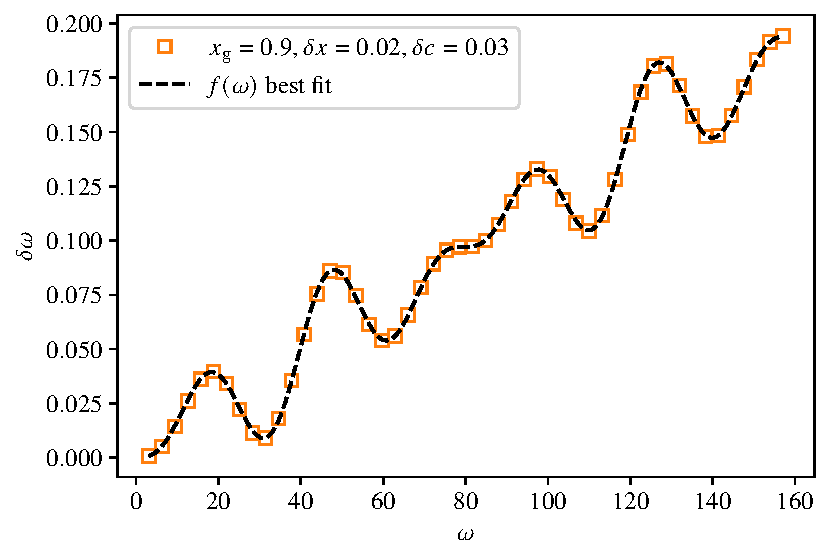
\includegraphics{figures/glitch-1d-fit.pdf}
    \caption{Best fit of Equation \ref{eq:1d-domega-func} to \(\delta\omega_n\) for \(n=1,\dots,50\), \(L=1\), and \(c=1\).}
    \label{fig:1d-fit}
\end{figure}

It would not be hard to believe that a similar oscillation could be found in the mode frequencies of a star, although its structure is more complicated. We showed that fitting to \(\delta\omega\) we may can recover properties of a glitch. In the next section, we will explore glitches in stars.

% NOTES: Go slowly through this. The next step is to fit a simple mode to theses oscillations and show that we can find x0 and dx. And show how the amplitude scales with dc.

% NOTES: When it comes to fitting the helium glitch, consider first fitting a GP to the modes with a free noise term. Fix the kernel scale to a series of values and show that we can see the glitch in the residuals. Of course, this leaves the question of what kernel scale to use. Well, we could just model everything at once!

\section{Acoustic glitches in stars}

\subsection{Helium glitch}\label{sec:helium-glitch}

Where does the helium glitch come from?

In a star, gamma is effected by the ionisation of elements. This effects the speed of sound,

\begin{equation}
    c = \sqrt{\gamma \frac{p}{\rho}},
\end{equation}

where \(p\) is pressure, \(\rho\) is density, and \(\gamma\) is the first adiabatic exponent,

\begin{equation}
    \gamma \equiv \Gamma_1 = \left( \frac{\partial \ln p}{\partial \ln \rho} \right)_s,
\end{equation}

where \(s\) is specific entropy.

We can simplify the problem to consider a star of just hydrogen and helium. Using the approach of Houdeyer we can derive an apporximation for \(\gamma\) in terms of temperature and density in the star

Reference Houdeyer's paper with plots to show the depression in the first adiabatic exponent with temperature and pressure. 

\begin{figure}
    \centering
    \includegraphics{example-image-a}
    \caption{Multi-panel figure showing \(\gamma\) as a function of \(\rho\) and \(T\) for different values of helium abundance.}
    \label{fig:gamma-temp-density}
\end{figure}

Now we look at the radial order kernels and how they are sensitive to different region


One approach is in Houdek and Gough, to take a perturbation in gamma and propagate this to a perturbation in frequency.

\subsection{Base of the convective zone glitch}\label{sec:bcz-glitch}

Other glitches are present. Sharp structure variation

\section[Modelling the glitch]{Modelling glitches in stellar oscillations}


\subsection{Gaussian processes }\label{sec:glitch-gp}

